\subsection{Halved Archetypal Model}
\label{sec:add.add.halved}

\hl{
	This section introduces the halved archetypal model.
	First, the motivation and a definition is given.
	After that, this section explains how this halved archetypal model is used to describe the \gls{pal} structures in the archetypal model.
}

\subsubsection{Motivation and Definition}

\hl{
	Since the archetypal model is a circle map, it can also be looked at as an infinite map.
}
Let $m$ be the archetypal model.
We know the model $m$ maps an input $x$ to $f(x) \mod 1$, meaning that if the output $f(x)$ is greater or equal to 1 we subtract 1 from it until it is in the range $[0, 1)$.
Similarly, we add 1 to it if it is smaller than 0 until it is in the desired range.
Now instead of confining the model to the domain of $[0, 1)$, we think of it repeating infinitely in both directions.
This process is called lifting of circle maps and is described by \Citeauthor{devaney2021introduction} in his book~\cite{devaney2021introduction}.
We can achieve this by mapping $T^m: x \mapsto f(x - \lfloor x \rfloor)$.
This trick maps any input $x \in \mathbb{R}$ into the domain $[0, 1)$ of the archetypal model $m$ and causes $T^m$ to repeat infinitely.
$T^m$ is now a lift of the model $m$ in the domain of all real numbers $\mathbb{R}$.
\Cref{fig:add.halved.lift} illustrates this concept for the cycle in the parameter region $P^{14}_3$.
\hl{
	The archetypal model in the lifted archetypal model is marked with a blue square.
	These blue squares repeat infinitely in each direction.
}
One can see that the branch $f_\D$ is outside the blue square at its right edge.
This is because it was cut off and continued at the bottom of the square \hl{in the archetypal model}, due to the $\mod 1$ operation.

\begin{figure}
	\centering
	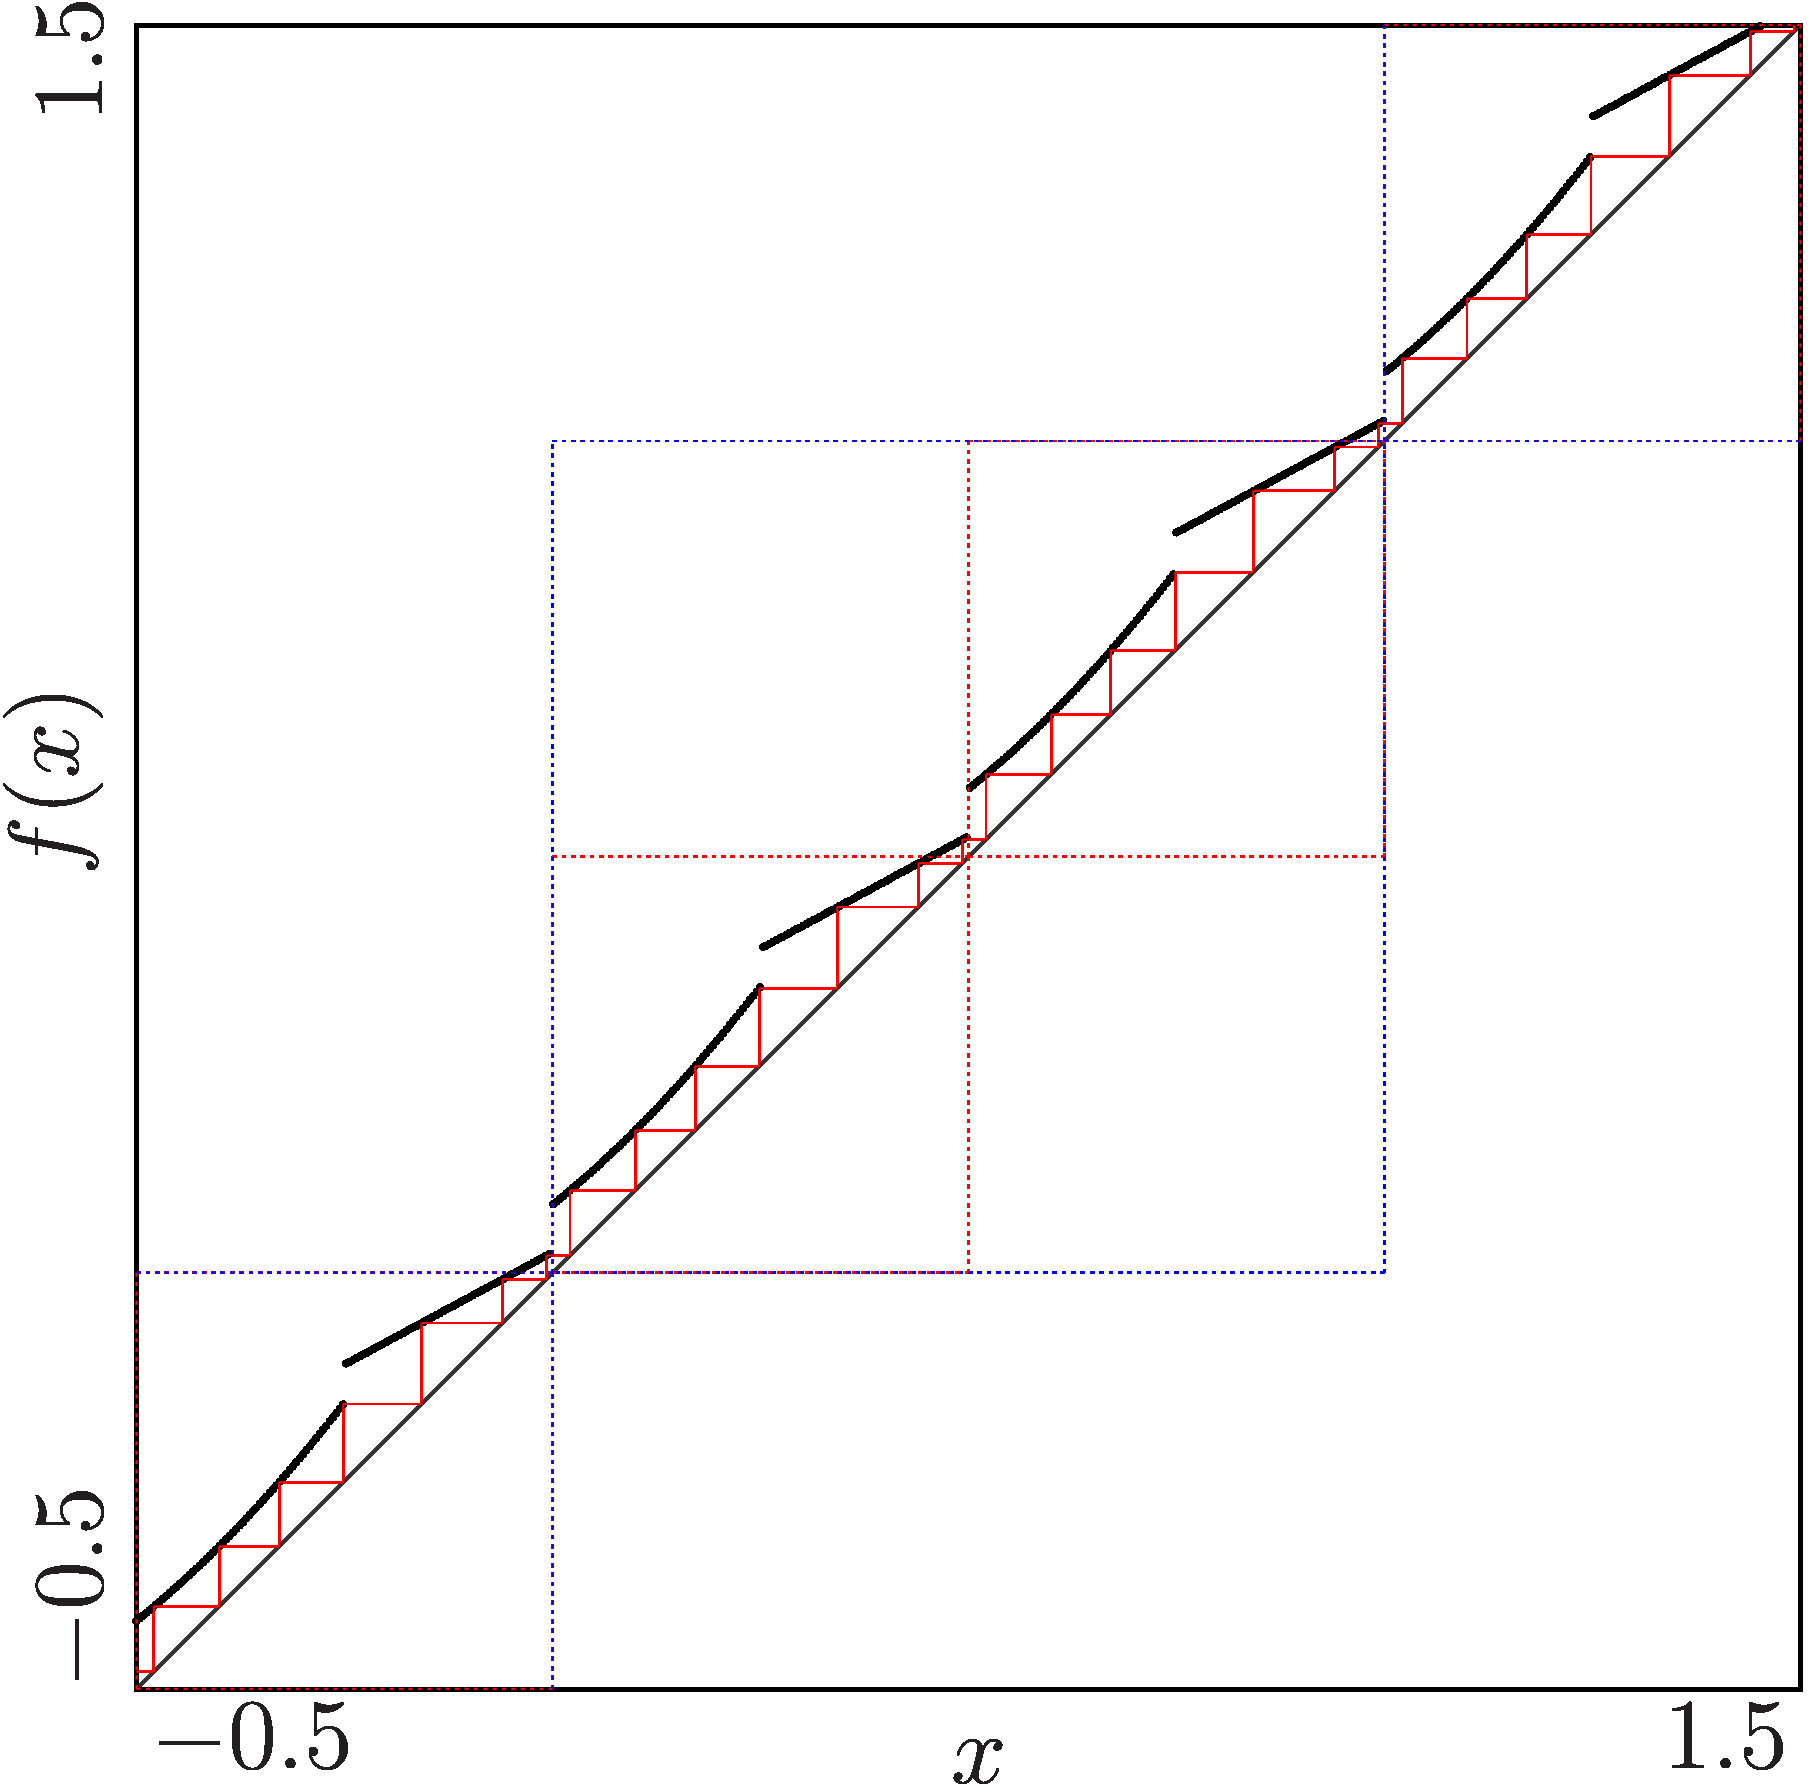
\includegraphics[width=.7 \textwidth]{../Figures/7/7.18/result.png}
	\caption{Illustration of the lifted archetypal model}
	\label{fig:add.halved.lift}
\end{figure}

In this model, there are no cycles that have multiple rotations.
Instead, the cycles that had multiple rotations in the archetypal model, manifest as a sequence of different blocks of the archetypal model.
Meaning, for the example $P^{14}_3$, the same blocks of $\A^4\B^3\C^4\D^3$ are repeating infinitely.
But for an example with multiple rotations, such as $\A\B\C\D\A^2\B^2\C^2\D^2$, the blocks will not all be the same.
Instead, the blocks $\A\B\C\D$ and $\A^2\B^2\C^2\D^2$ will be alternating.

Now we will take advantage of the symmetry in the model function $f$ of the archetypal model.
Since $f\left(x + \frac{1}{2}\right) \equiv f(x) + \frac{1}{2} \mod 1$, we can split the lifted model $T^m$ into smaller blocks of size $\frac{1}{2}$.
The function of the infinite model repeats in these smaller blocks.
These blocks are marked red in \Cref{fig:add.halved.lift}.
The red blocks represent the halved model, it is the smallest repeating part of the lifted model $T^m$.
Basically we choose the smallest model, of which $T^m$ is a lift.
This happens to be exactly our model $m$ folded in half.
So the halved archetypal model \hl{is defined as $x_{n+1} = g(x_n) \mod \frac{1}{2}$}, where $g(x)$ is the same as in the archetypal model defined in \Cref{sec:setup.arch.definition}.

\subsubsection{Utility in Explaining the \Glsentrylong{pal} Structures}

\Cref{fig:add.halved.hor.2D} \hl{shows a 2D scan of the periods associated with parameter regions in the halved archetypal model in the same parameter ranges used for the 2D period scan of the horizontally oriented \gls{pal} structures in} \Cref{fig:add.add.like.hor.2D}.
The red arrow indicates the parameter range for the 1D period scan in \Cref{fig:add.halved.hor.1D}.
The 1D scan shows that the periods in this structure add up as we would expect in \gls{pa} structures.

\begin{figure}
	\centering
	\subfloat[2D period scan]{
		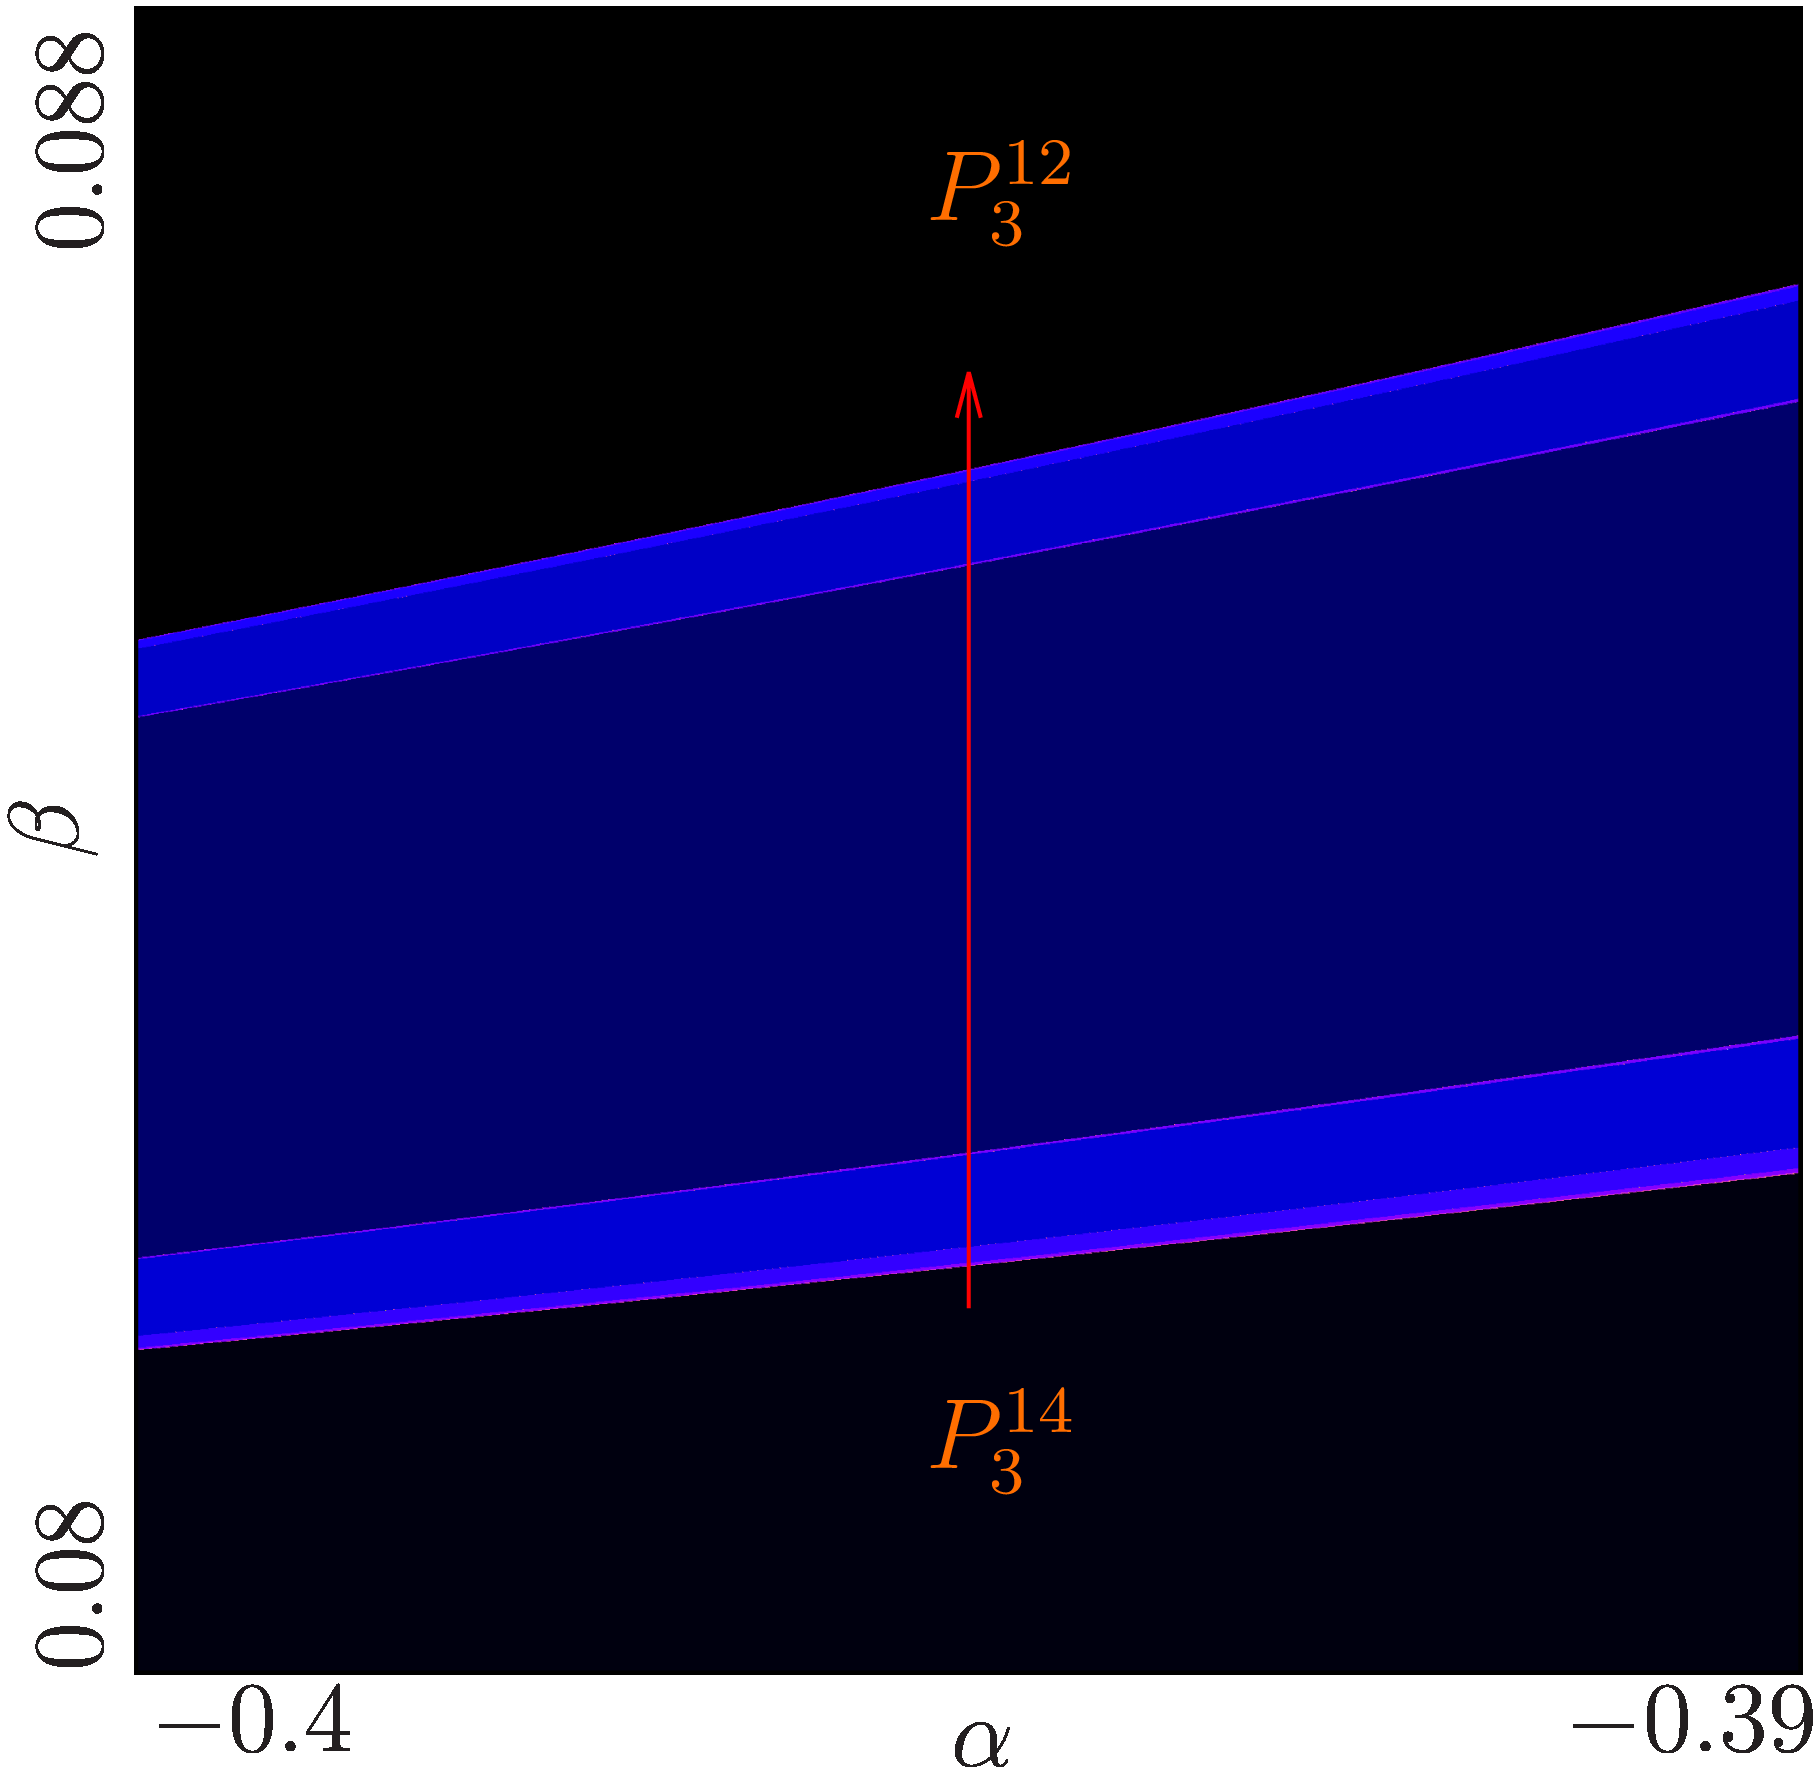
\includegraphics[width=.45 \textwidth]{../Figures/7/7.19a/result.png}
		\label{fig:add.halved.hor.2D}
	}
	\subfloat[1D period scan]{
		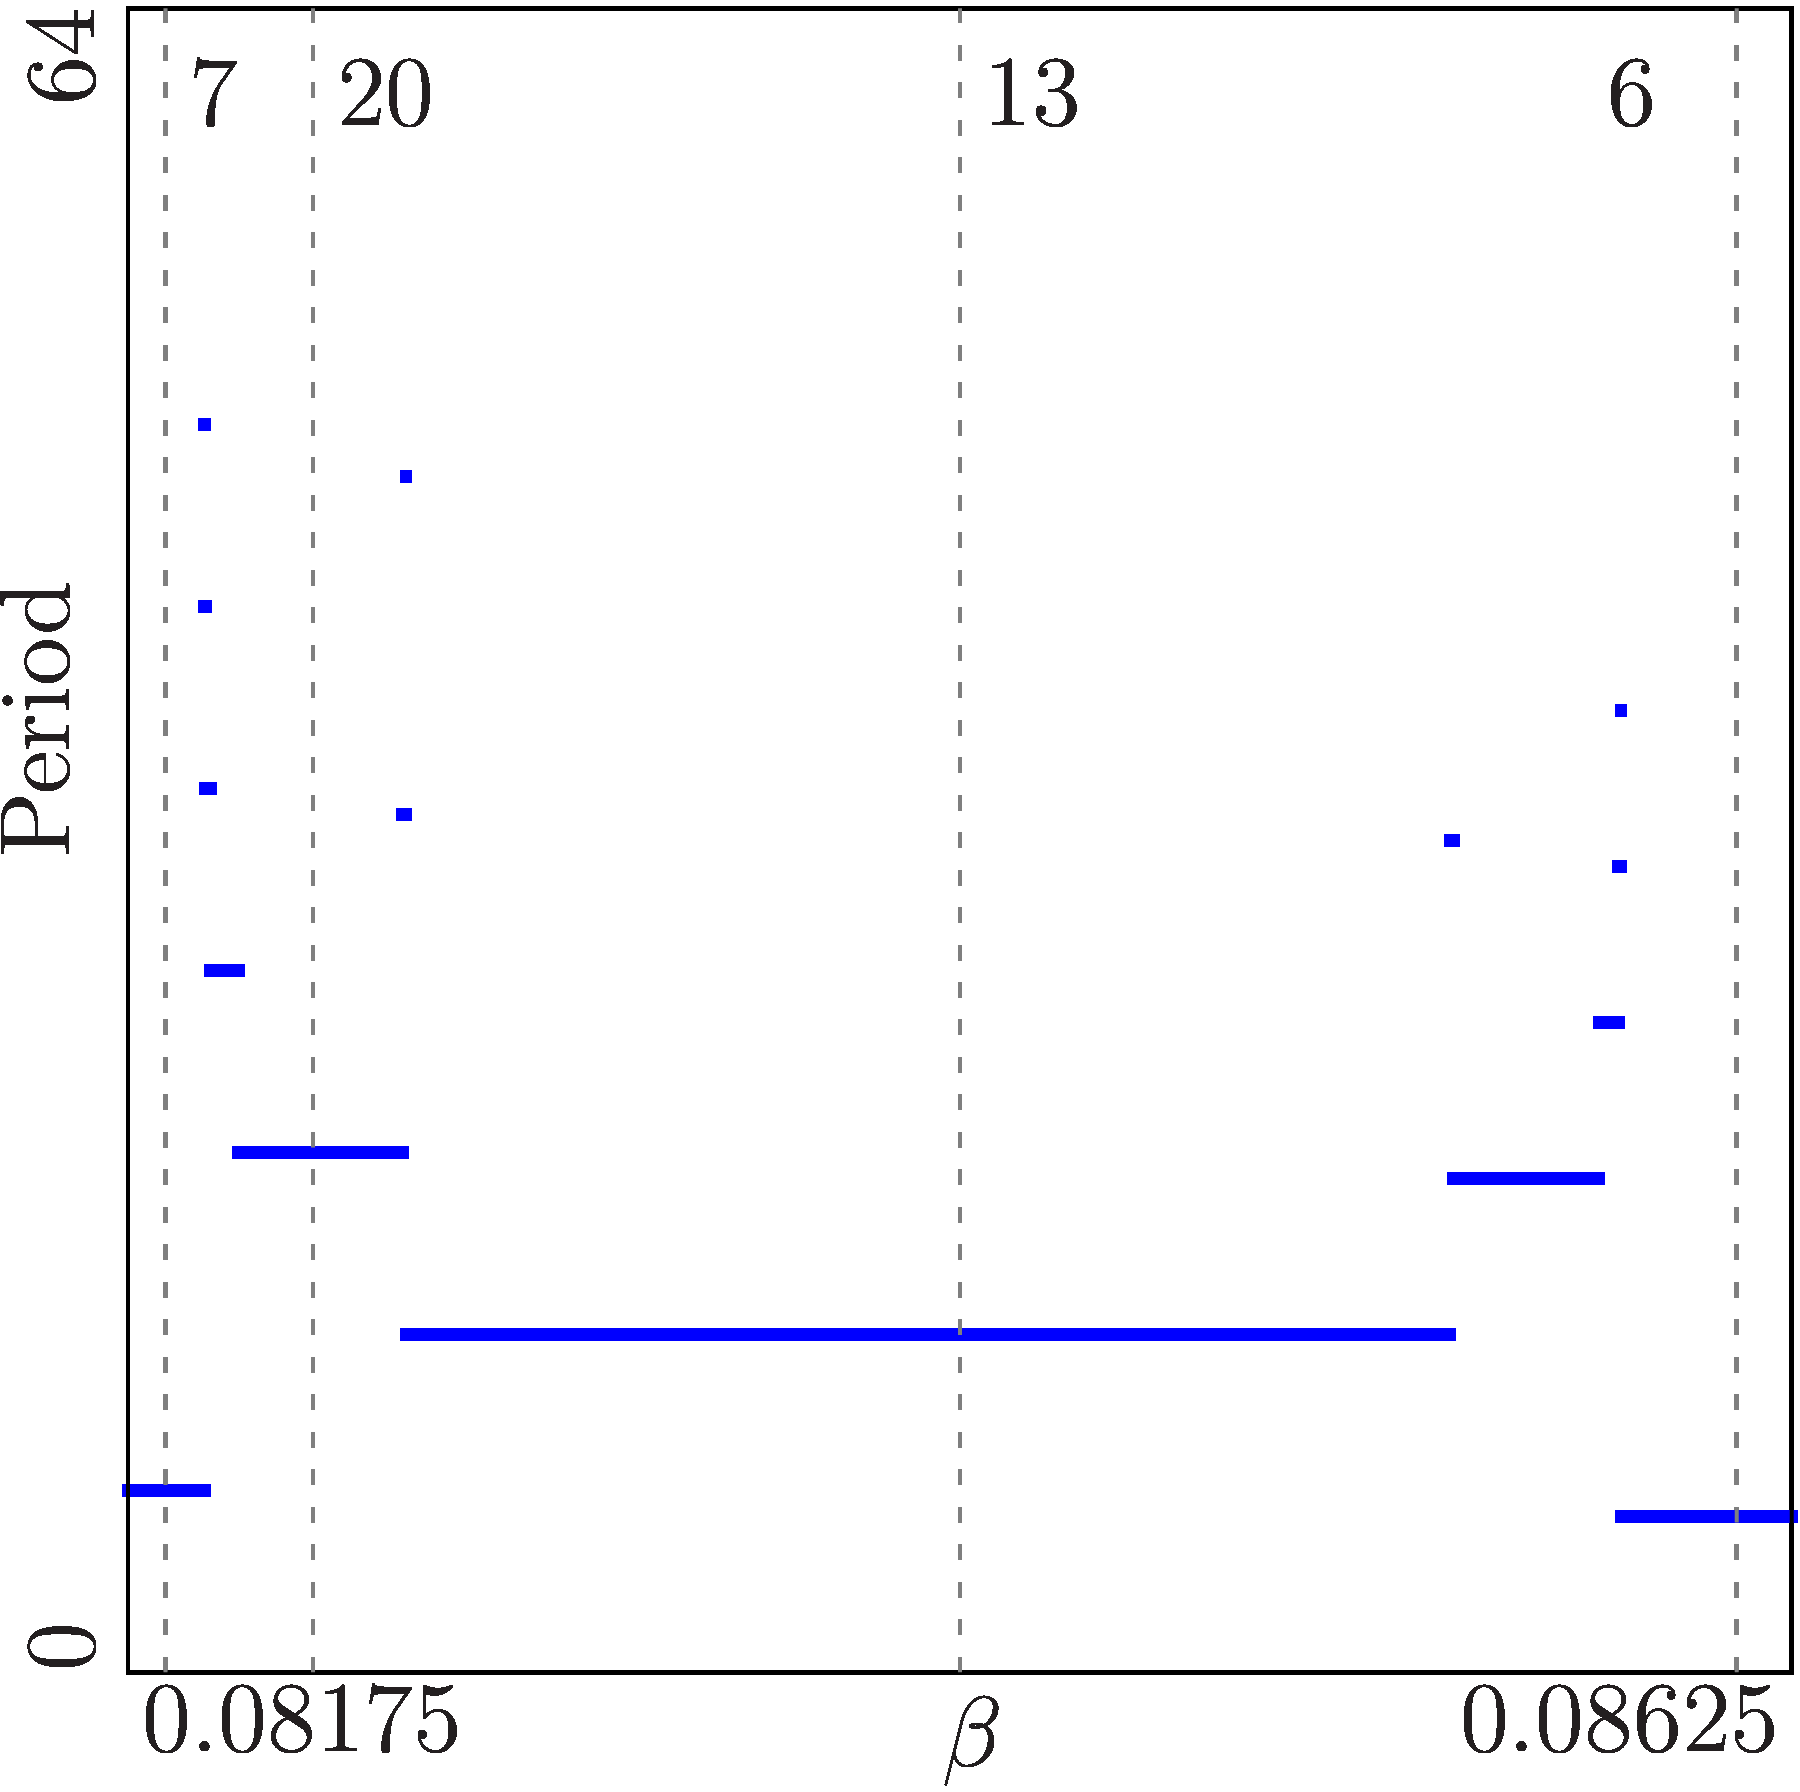
\includegraphics[width=.45 \textwidth]{../Figures/7/7.19b/result.png}
		\label{fig:add.halved.hor.1D}
	}
	\caption[2D and 1D period scans of a horizontal period-adding structure in the halved increasing archetypal model]{
		2D and 1D period scans of a horizontal \gls{pa} structure in the halved increasing archetypal model.
		The fixed parameters are $a_L = 1, b_L = 0.8,$ and $g_R\left(\frac{1}{2}\right) = \frac{1}{2} + \frac{1}{40}$.
		(a) shows the 2D period scan where the parameters $\alpha = g_R\left(\frac{1}{4}\right)$ and $\beta = c_L$ are varied.
		The small arrow indicates the parameter range for the 1D period scan in (b).
		Here, only $\beta$ is varied.
		The numbers at the top mark the periods at the corresponding value for $\beta$.
	}
	\label{fig:add.add.halved.hor}
\end{figure}

\hl{
	As in the previous sections, the symbolic sequences of the cycles associated with the parameter regions in this structures are examined.
}
\Cref{fig:halved.hor.tree} shows the Farey-tree with the symbolic sequences associated with the parameter regions of this structure.
One can see that the symbolic sequence of a child node is the concatenation of the symbolic sequences of the parent nodes, as we would expect from \gls{pa} structures.
It turns out that the hybrid parameter region $\left[P^{14}_3 \mid P^{12}_3\right]$ was also part of the horizontal \gls{pal} structure described in \Cref{sec:add.add.like}.
And the \gls{pal} structures in the archetypal model are consequences of the \gls{pa} structures in the halved archetypal model.

\begin{figure}
	\centering
	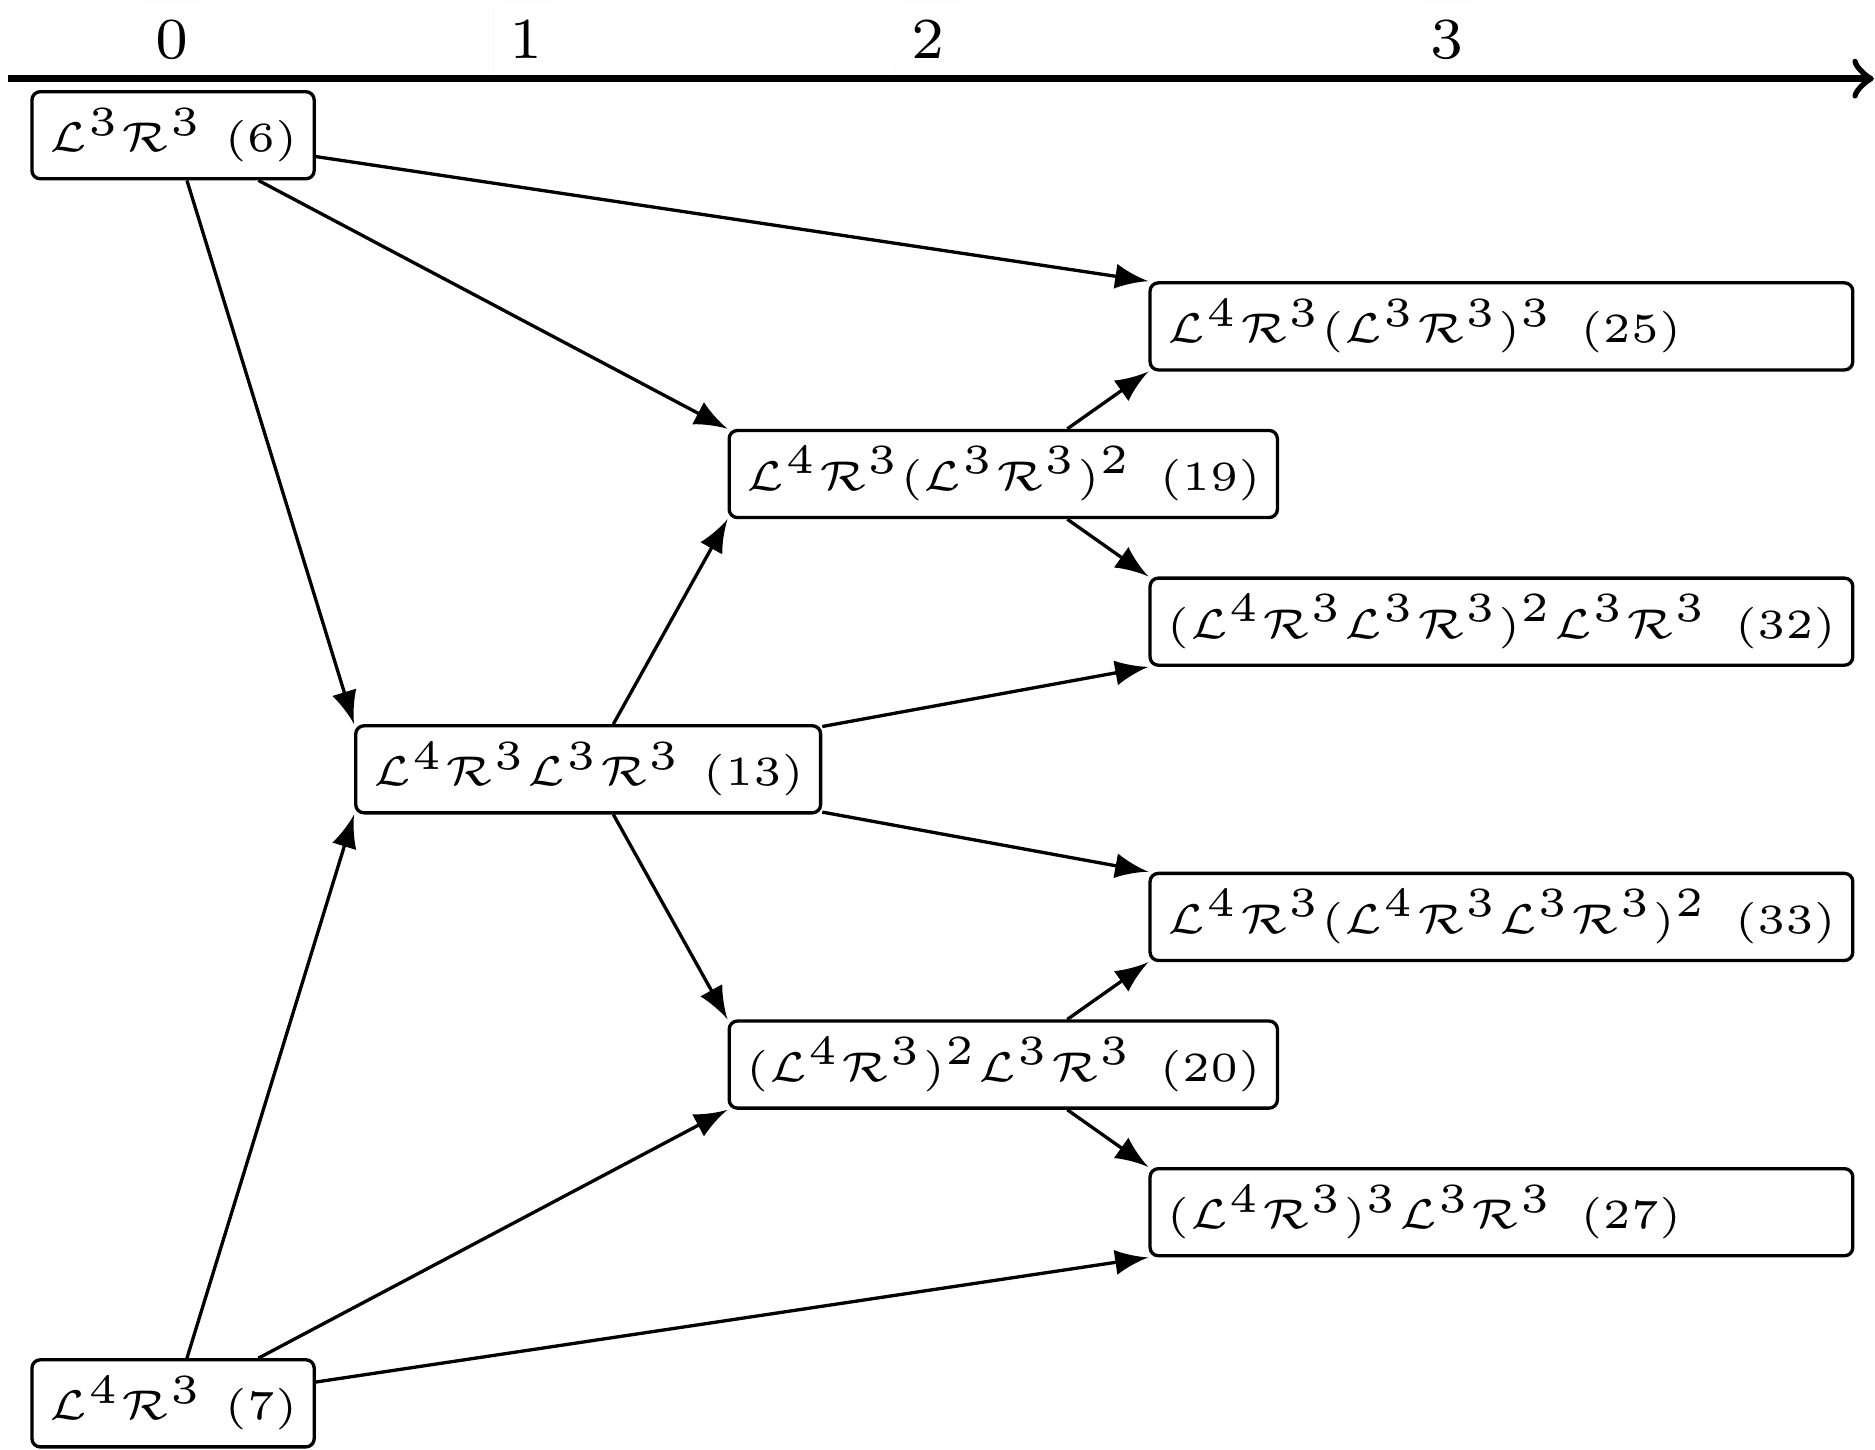
\includegraphics[width=.7 \textwidth]{../Figures/7/7.20/adding.png}
	\caption[Farey-tree with the symbolic sequences of a horizontal \glsentrylong{pa} structure]{
		Farey-tree with the symbolic sequences associated with the parameter regions of the horizontal \gls{pa} structure marked with a red arrow in \Cref{fig:add.halved.hor.2D} up to three levels.
	}
	\label{fig:halved.hor.tree}
\end{figure}

\hl{
	The numerical evidence shows that the \gls{pa} structures in the halved archetypal model manifest as \gls{pal} structures in the archetypal model.
	And the rules for the symbolic sequences of parameter regions in \gls{pa} structures are well known.
	By formulating an algorithm that can translate symbolic sequences between the halved archetypal model and the archetypal model, one can generate the symbolic sequences of any \gls{pal} structure without the need for simlulating the archetypal model in every parameter region of the \gls{pal} structure.
	Furthermore, with such an algorithm, one can derive rules for the \gls{pal} structures in the archetypal model from the rules for \gls{pa} structures.
	The rules include rules for the periods, symbolic sequences, multistability, and even rotation numbers of the cycles associated with the parameter regions.
}

\hl{
	The next section introduces such algorithms and formulates some regularities in the translation of symbolic sequences.
	With these algorithms and regularities, the rules for \gls{pal} structures in the archetypal model are derived later.
}
